$y=(x-2)^2$ can be written as,
\begin{align} \label{eq:solutions/1/13/eq:eq_1}
    x^2-4x-y+4=0
\end{align}
From \eqref{eq:solutions/1/13/eq:eq_1}, 
\begin{align} 
    \vec{V} = \myvec{1 & 0 \\ 0 & 0};\vec{u} = \myvec{-2 \\ -\frac{1}{2}};f=4 \label{eq:solutions/1/13/eq:eq_2} \\
    \mydet{V} = \mydet{1 & 0 \\ 0 & 0} = 0 \label{eq:solutions/1/13/eq:eq_3}
\end{align}
\eqref{eq:solutions/1/13/eq:eq_3} implies that the curve is a parabola. Now, finding the eigen values corresponding to the $\vec{V}$,
\begin{align}
    \mydet{V-\lambda I} = 0 \nonumber \\
    \mydet{1-\lambda & 0 \\ 0 & -\lambda} = 0 \nonumber \\
    \implies \lambda=0,1 \label{eq:solutions/1/13/eq:eq_4}
\end{align}
Calculating the eigenvectors corresponding to $\lambda=0,1$ respectively,
\begin{align}
    \vec{V}\vec{x} = \lambda\vec{x} \nonumber 
\end{align}
\begin{align}
    \myvec{1 & 0 \\ 0 & 0}\vec{x} = 0;\implies \vec{p}_1 = \myvec{0 \\ 1} \label{eq:solutions/1/13/eq:eq_5} \\
    \myvec{0 & 0 \\ 0 & -1}\vec{x} = 0;\implies \vec{p}_2 = \myvec{1 \\ 0} \label{eq:solutions/1/13/eq:eq_6}
\end{align}
By Eigen decomposition on $\vec{V}$,
\begin{align}
    \vec{V} = \vec{P}\vec{D}\vec{P}^T \nonumber \\
    where, \vec{P} = \myvec{\vec{p}_1 & \vec{p}_2} = \myvec{0 & 1 \\ 1 & 0} \label{eq:solutions/1/13/eq:eq_7} \\
    \vec{D} = \myvec{\lambda_1 & 0 \\ 0 & \lambda_2} = \myvec{0 & 0 \\ 0 & 1} \label{eq:solutions/1/13/eq:eq_8}
\end{align}
To find the vertex of the parabola,
\begin{align}
    \myvec{\vec{u}^T+\eta \vec{p}_1^T \\ \vec{V}}\vec{c} = \myvec{-f \\ \eta \vec{p}_1-\vec{u}} \label{eq:solutions/1/13/eq:eq_9} \\
    where, \eta = \vec{u}^T\vec{p}_1 = -\frac{1}{2} \label{eq:solutions/1/13/eq:eq_10}
\end{align}
Substituting values from \eqref{eq:solutions/1/13/eq:eq_2}, \eqref{eq:solutions/1/13/eq:eq_5} and \eqref{eq:solutions/1/13/eq:eq_10} in \eqref{eq:solutions/1/13/eq:eq_9}, 
\begin{align}
    \myvec{-2 & -1 \\ 1 & 0 \\ 0 & 0}\vec{c}=\myvec{-4 \\ 2 \\ 0} \label{eq:solutions/1/13/eq:eq_11}
\end{align}
Removing last row and representing \eqref{eq:solutions/1/13/eq:eq_11} as augmented matrix and then converting the matrix to echelon form,
\begin{align}
    \myvec{-2 & -1 & -4 \\ 1 & 0 & 2} \xleftrightarrow[]{R_1\leftarrow\frac{R_1}{-2}} \myvec{1 & \frac{1}{2} & 2 \\ 1 & 0 & 2} \xleftrightarrow[]{R_2\leftarrow R_2-R_1} \nonumber \\
    \myvec{1 & \frac{1}{2} & 2 \\ 0 & -\frac{1}{2} & 0} \xleftrightarrow[]{R_2\leftarrow(-2R_2)} \myvec{1 & \frac{1}{2} & 2 \\ 0 & 1 & 0} \xleftrightarrow[]{R_1\leftarrow R_1-\frac{R_2}{2}} \nonumber
\end{align}
\begin{align}
    \myvec{1 & 0 & 2 \\ 0 & 1 & 0} \label{eq:solutions/1/13/eq:eq_12}
\end{align}
From \eqref{eq:solutions/1/13/eq:eq_12} it can be observed that,
\begin{align}
    \vec{c} = \myvec{2 \\ 0} \label{eq:solutions/1/13/eq:eq_13}
\end{align}
Direction vector of the chord joining A(4,4) and B(2,0) can be calculated as,
\begin{align}
    \vec{m} = \vec{A} - \vec{B} = \myvec{4 \\ 4} - \myvec{2 \\ 0} = \myvec{2 \\ 4} = 2\myvec{1 \\ 2} \nonumber
\end{align}
\begin{align}
    \implies \vec{m} = \myvec{1 \\ 2} \label{eq:solutions/1/13/eq:eq_14}
\end{align}
We know that,
\begin{align} \label{eq:solutions/1/13/eq:eq_15}
    \vec{m}^T\vec{n} = 0; \implies \vec{n} = \myvec{2 \\ -1} 
\end{align}
To find the point of contact $\vec{q}$, which is intersection point for normal of the chord AB and also tangent of the curve,
\begin{align}
    \myvec{\vec{u}^T+\kappa\vec{n}^T \\ \vec{V}}\vec{q}=\myvec{-f \\ \kappa\vec{n} - \vec{u}} \label{eq:solutions/1/13/eq:eq_16} \\
    where, \kappa = \frac{\vec{p_1}^T\vec{u}}{\vec{p_1}^T\vec{n}} = \frac{1}{2} \label{eq:solutions/1/13/eq:eq_17}
\end{align}
Substituting the values from \eqref{eq:solutions/1/13/eq:eq_2},\eqref{eq:solutions/1/13/eq:eq_15} and \eqref{eq:solutions/1/13/eq:eq_17} in \eqref{eq:solutions/1/13/eq:eq_16},
\begin{align}
    \myvec{-1 & 1 \\ 1 & 0 \\ 0 & 0}\vec{q} = \myvec{-4 \\ 3 \\ 0} \label{eq:solutions/1/13/eq:eq_18}
\end{align}
Removing last row and representing \eqref{eq:solutions/1/13/eq:eq_18} as augmented matrix and then converting the matrix to echelon form,
\begin{align}
    \myvec{-1 & -1 & -4 \\ 1 & 0 & 3} \xleftrightarrow[]{R_1\leftarrow(-R_1)} \myvec{1 & 1 & 4 \\ 1 & 0 & 3} \xleftrightarrow[]{R_2\leftarrow R_2-R_1} \nonumber \\
    \myvec{1 & 1 & 4 \\ 0 & -1 & -1} \xleftrightarrow[]{R_2\leftarrow(-R_2)} \myvec{1 & 1 & 4 \\ 0 & 1 & 1} \xleftrightarrow[]{R_1\leftarrow R_1-R_2} \nonumber 
\end{align}
\begin{align}
    \myvec{1 & 0 & 3 \\ 0 & 1 & 1} \label{eq:solutions/1/13/eq:eq_19}
\end{align}
From \eqref{eq:solutions/1/13/eq:eq_19}, it can be observed,
\begin{align}
    \vec{q} = \myvec{3 \\ 1}
\end{align}
which is the required point of contact
\begin{figure}[ht!]
    \centering
    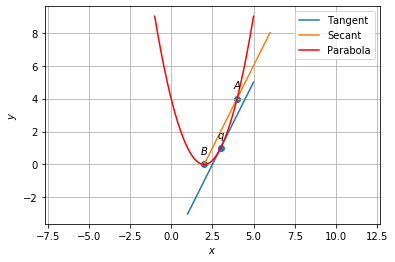
\includegraphics[width=\columnwidth]{./solutions/conics/1/13/Assignment_7_Plot.png}
    \caption{Parabola with AB as chord, a tangent parallel to the chord}
    \label{eq:solutions/1/13/Fig:1}
\end{figure} 
